Chaque joueur peut choisir son contrôleur de jeu via les options du menu. Il a le choix entre ces différents périphériques :

\begin{itemize}
    \item Clavier,
    \item Joystick,
    \item Wiimote.
\end{itemize}

\vspace{0.5cm}

Chaque joueur a 7 touches utilisables pendant le jeu, afin de se déplacer dans les 4 directions (haut, bas, gauche, droite), ainsi que deux touches d'action afin de poser des bombes et d'effectuer une action secondaire (pour utiliser le détonateur ou bien poser une mine par exemple), et une touche de pause.
	
\subsection{Clavier}

Il est possible de paramétrer les différentes commandes du jeu en passant par le menu. Les commandes de jeu sont représentées sur l'image page suivante.

\begin{figure}
    \begin{center}
	    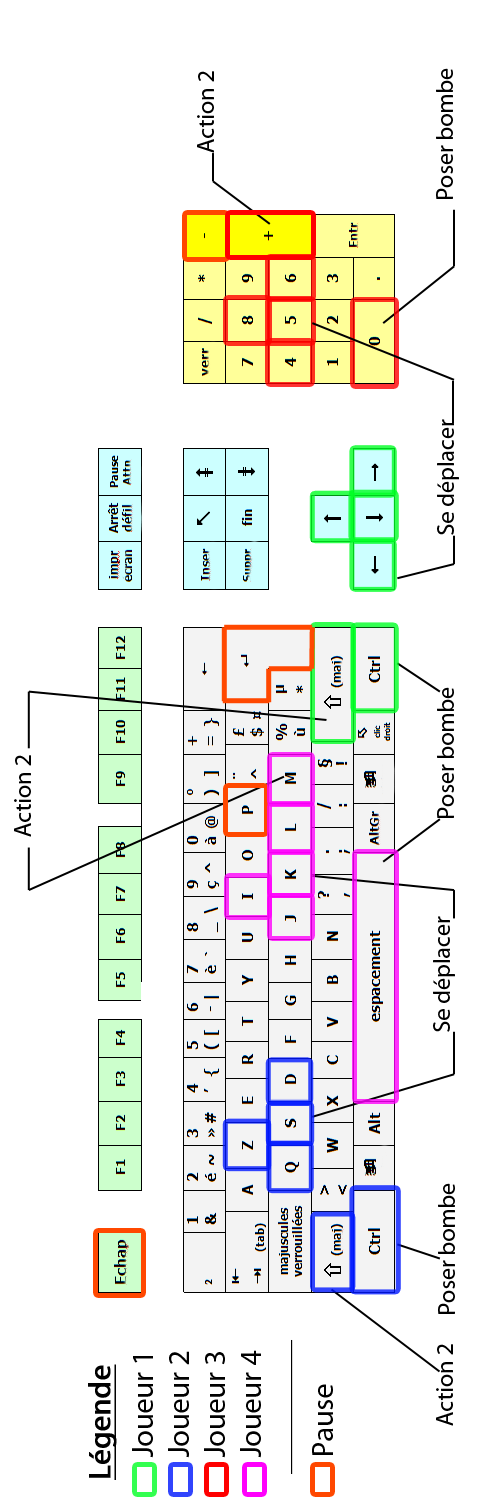
\includegraphics[height=520pt]{images/clavier}
    \end{center}
    \caption{Disposition des touches par défaut du clavier}
\end{figure}

\subsection{Joystick}

Le programme permettra également la prise en charge des autres contrôleurs de jeux PC de type joystick. Comme le clavier, il sera possible de paramétrer les différentes commandes du jeu en passant par le menu. Par défaut ce sont les suivantes :

\begin{center}
	\begin{tabular}{|c|c|}
		\hline
			%\rowcolor{blueTab}
			\textbf{Action} & \textbf{Touches} \\
		\hline
		Se déplacer & Pad directionnel \\
		\hline
		Poser une bombe & Bouton 1\\
		\hline
		Action 2 & Bouton 2\\
		\hline
		Pause & Bouton 3\\
		\hline
	\end{tabular}
\end{center}


\subsection{Wiimote}

Tout comme les joysticks, le programme permettra de jouer avec une Wiimote (manette de la console Wii). Le jeu ne requiert pas l'utilisation de l'accessoire Nunchuck. Les commandes de jeu sont les suivantes et ne peuvent pas être modifiées :

\begin{center}
	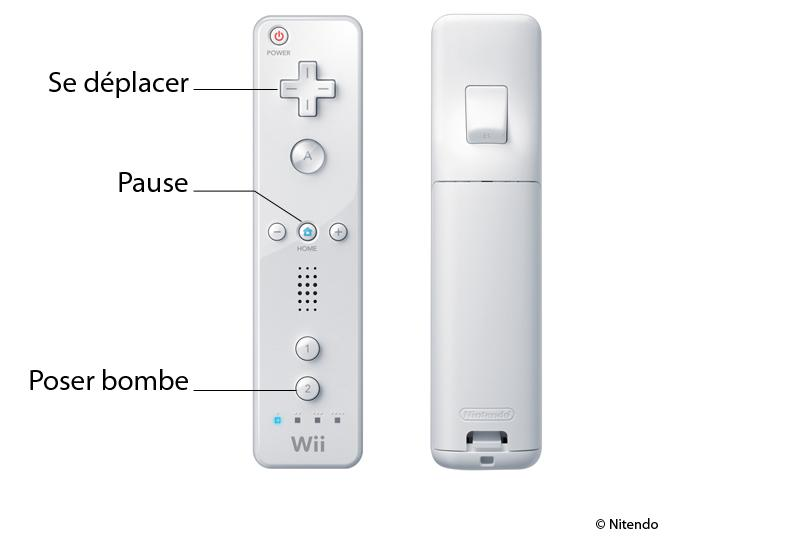
\includegraphics[scale=1.3]{images/wiimote}
\end{center}